\section{Corriente Eléctrica}

Para los casos en que las carga no son estáticas, se llama corriente eléctrica al flujo de una distribución continua de carga eléctrica.

\subsection{Intensidad}

La intensidad de corriente eléctrica es la carga que atraviesa una superficie en un instante.

\[I = \frac{dQ}{dt}\]

\begin{figure}[H]
    \centering
    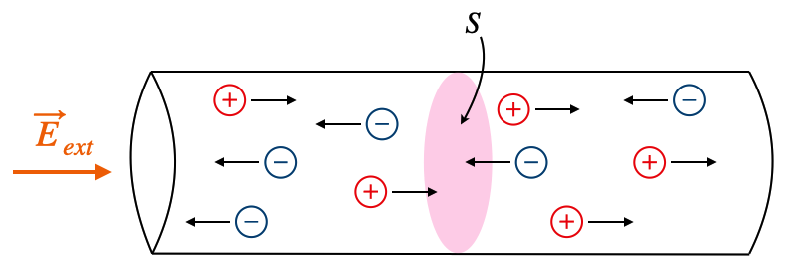
\includegraphics[width=0.49\textwidth]{Corriente/corriente.png}
    \caption{Visualización corriente eléctrica.}
\end{figure}

Considerando una densidad de carga eléctrica $\rho(\Vec{r},t)$ que se desplaza con velocidad $\Vec{v}(\Vec{r},t)$ y pasa por una superficie $\Vec{S}$, la cantidad de carga $dQ$ que atraviesa un elemento de superficie $d\Vec{S}$ durante un intervalo de tiempo $dt$ es aquella contenida en un volumen de ancho $\Vec{v}dt$ y sección $d\Vec{S}$

\[dQ = \rho\Vec{v}dt\cdot d\Vec{S}\]
\bigbreak

de modo que

\[Q = \int\rho\Vec{v}\,dt\cdot d\Vec{S}\]

\subsection{Densidad de Corriente}

Se define la densidad de corriente eléctrica como la cantidad de corriente por área

\[\Vec{J}=\rho\Vec{v}\]
\bigbreak
Para una superficie regular orientable $\mathcal{S}$, se verifica que

\[I = \int_\mathcal{S} \Vec{J}\cdot d\Vec{S}\]
\bigbreak

Las cargas positivas se mueven en el sentido de $\Vec{J}$ y las cargas negativas en el sentido opuesto. Esto implica que si $I > 0$, las cargas positivas atraviesan $\mathcal{S}$ en el sentido de la orientación de la superficie, y si $I < 0$, las cargas positivas atraviesan $\mathcal{S}$ en el sentido de opuesto a su orientación.

\subsection{Principio de Conservación}

El principio de conservación de carga eléctrica indica que no existe creación ni destrucción de las cargas eléctricas.

\subsection{Ley de Continuidad}

Sea $\Omega$ la región del espacio contenida por una superficie cerrada $\partial\Omega$, se tiene que

\begin{equation}
\begin{split}
    Q &= \int_\Omega\rho\, d\V\\
    I &= \frac{dQ}{dt} =
    \int_\Omega\frac{\partial\rho}{\partial t}\,d\V\\
\end{split}
\nonumber
\end{equation}

Estableciendo positiva la norma exterior, si la carga ingresa a $\Omega$, $I$ es positiva y $\Vec{J}$ apunta al interior, si la carga sale de $\Omega$, $I$ es negativa y $\Vec{J}$ apunta al exterior. En ambos casos casos para que el signo de $I$ y $\Vec{J}\cdot d\Vec{S}$ coincidan, se debe tomar la norma negativa, sin embargo lo común es utilizar la norma exterior por lo que se escribe 

\[I = -\oint_{\partial\Omega}\Vec{J}\cdot d\Vec{S}=-\int_\Omega \nabla\cdot \Vec{J}\,d\V\]
\bigbreak
Con esto, se obtiene que

\[\int_\Omega\frac{\partial\rho}{\partial t}\,d\V=
-\int_\Omega \nabla\cdot \Vec{J}\,d\V\]
\bigbreak

de lo cual se deduce la ecuación de continuidad:

\[\frac{\partial\rho}{\partial t}+\nabla\cdot\Vec{J}=0\]

la ecuación de continuidad expresa que si la carga aumenta en una región, disminuye en otra.

\subsection{Régimen Estacionario}

Se dice que una corriente continua está en un régimen estacionario si se verifica que
% no se si es que pueden ser estacionarias o todo corriente continua es estacionaria

% Tengo entendido que continua no implica estacionaria, estacionaria es que la cantidad de carga en un sector no cambia con el tiempo. Mientras que continua es que no hay interrupciones (o cortes bruscos) en el flujo de la corriente
\[\frac{\partial\rho}{\partial t}=\nabla\cdot\Vec{J}=0 \quad \wedge \quad \nabla\times\Vec{E}=0\]

El rotor nulo de $\Vec{E}$ permite que el potencial electrostático siga siendo valido para la corriente continua.

\subsection{Primera Ley de Kirchhoff}

En un régimen estacionario la intensidad de corriente total de un nodo de un circuito en nula. Esto es, para un nodo conectado a $n$ conductores encerrado en un volumen $\Omega$ arbitrario, se verifica que

\[\int_\Omega\nabla\cdot\Vec{J}\,d\V=\oint_{\partial \Omega}
\Vec{J}\cdot d\Vec{S}=\sum_{i=1}^n\int_{S_i}
\Vec{J}_i\cdot d\Vec{S}=\sum_{i=1}^n I_i = 0\]

donde $S_i$ es la sección en la que intersectan el conductor $i$ con $\partial\Omega$. La primera ley de Kirchhoff implica que, siempre que una corriente entra a un nodo otra sale y no hay acumulación de carga.

\subsection{Ley de Ohm}

En un conductor óhmico o lineal se verifica que la densidad de corriente y el campo eléctrico son proporcionales.

\[\Vec{J} = g\Vec{E}\]

donde $g$ es la conductividad del material. A $\eta=\frac{1}{g}$ se le llama resistividad.\\

\subsubsection{Resistencia Eléctrica}

Se define la resistencia eléctrica, $R$, a través de la relación
\[V = IR\]
donde $V$ es la diferencia de potencial. Esta depende de la conductividad del material y de los parámetros geométricos del sistema
\[R = \abs{\frac{V}{I}} = \abs{\frac{\int \Vec{E}\cdot\Vec{dl}}{\int g\Vec{E}\cdot \Vec{ds}}}\]\\
\hfill \\
\textbf{Resistencias en Serie:}

En un circuito, 2 resistencias están en paralelo si se conectan por uno de sus extremos. En un régimen estacionario, ambas comparten la misma intensidad de corriente, de modo que

\begin{equation}
\begin{split}    
    &V_A-V_B=R_1I\\
    &V_B-V_C=R_2I\\
    &V_A-V_C=(R_1+R_2)I\\
\end{split}
\nonumber
\end{equation}

de esto se deduce que la resistencia equivalente en serie es

\[R_{eq}=R_1+R_2\]
\hfill \\
\textbf{Resistencias en Paralelo:}

En un circuito, dos resistencias están en paralelo si se conectan por sus dos extremos. Ambas comparten la diferencia de potencial y, en un régimen estacionario, se cumple que

\[I=I_1+I_2\]

donde $I_1$ e $I_2$ son las intensidades de corriente que pasan por cada corriente e $I$ es la intensidad total. Con esto, se tiene que

\[R_1I_1=\Delta V=R_2\]

\[I = \Delta\lados{(}{\frac{1}{R_1}+\frac{1}{R_2}}\]

se concluye así que, para la resistencia equivalente en paralelo, se cumple que

\[\frac{1}{R_{eq}}=\frac{1}{R_1}+\frac{1}{R_2}\]

\indeciso{M}{

\subsubsection{Conductores perfectos}
\label{teo:conductores_perfectos}
Para conductores perfectos se tiene que $E = \eta J = 0$, incluso si hay flujo de corriente. En la práctica los metales son tan buenos conductores que el campo eléctrico necesario para hacer fluir corriente en ellos es despreciable. Por ello se puede tratar la conexión en cables que conectan como equipotenciales. Las resistencias, por otro lado, están hechas de materiales que son malos conductores.
% Griffiths, D. J. (2013). Introduction to Electrodynamics. Pearson. Páginas 296-297. 
}

\subsection{Ley y Efecto Joule}
Siempre que existe una corriente eléctrica, esta conlleva una perdida de energía, la cual se disipa en forma de calor y es irrecuperable. A este fenómeno se le conoce como efecto Joule.
\subsubsection{Ley de Joule }
La potencia eléctrica corresponde a la energía electrostática disipada por unidad de tiempo. De manera general se tiene
\[P = \deriv{U_e}{t} = \int\Vec{E}\cdot\Vec{J}\,d\V\]
Y para materiales lineales (con $\Vec{J} = g\Vec{E}$),
\[P = \int g\norma{E}^2\,d\V\]

Para casos en que existe una única diferencia de potencial se verifica que

\[P = I^2R = \frac{V^2}{R} = IV\]

Con $V$ la diferencia de potencial. La energía total disipada por el efecto Joule se puede obtener de la siguiente forma
\[U = \int_{t_0}^{t_1}\int_V(\Vec{E}\cdot \Vec{J})d\V dt\]
Donde $\Vec{J}$ y $\Vec{E}$ dependen tanto del posición $\Vec{r}$ y el tiempo $t$.\\% esto es consecuencia directa de la definición de potencia, no se si sea necesario ponerlo

% En sí no lo es, pero ayuda a aprender del término más rápido según yo. hace que no sea necesario 'descubrir' la consecuencia por ti mismo

\subsection{Condiciones de Borde}

Entre dos medios distintos y en contacto, se producen las siguientes condiciones de borde

\begin{itemize}
    \item \textbf{Tangencial:} $E_{1t}=E_{2t}$
    \item \textbf{Normal:} $J_{2n}-J_{1n}=-\parfrac{\sigma}{t}$
\end{itemize}

donde $\sigma$ es la densidad de carga de la interfase.

\subsection{Fuente de Potencial}

Se llama fuente de potencial a un dispositivo que genera una diferencia de potencial entre dos puntos. A cada fuente se asocia una resistencia interna, $R_i$, y una fuerza electromotriz. Las fuentes de potencial más comunes son las baterías.\\
Una fuente de potencial inyecta al sistema la energía que se pierde por el efecto Joule.

\subsubsection{Fuerza Electromotriz}

La fuerza electromotriz o f.e.m. corresponde a una diferencia de potencial intrínseca a la fuente, que produce una discontinuidad en el campo eléctrico. Esta se representa por $\mathcal{E}$ y se obtiene de la ecuación

\[V = \mathcal{E}-R_iI\]

con $V$ la diferencia de potencial generada por la fuente.

\newpage